\section{Appendix: StructFlow Details}
\label{app:compiler}

We provide the implementation details for Inference Alignment of a DAG.

\begin{figure*}[hbt!]
    \centering
    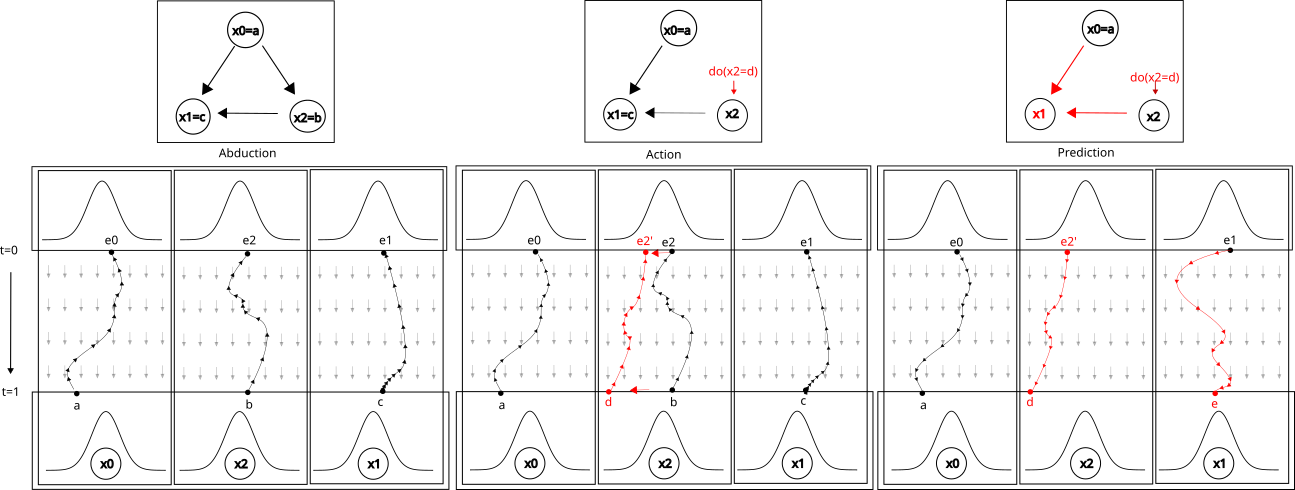
\includegraphics[width=\textwidth]{images/collider-counterfactual.png}
    \caption{\textbf{Counterfactual Inference via Flow Inversion.} To answer ``What would $Y$ have been if $X$ had been $x'$?'', we perform three steps. \textbf{(1) Abduction:} Integrate backward from the observation $(x, y)$ to recover the exogenous noise $u = (u_X, u_Y)$. \textbf{(2) Action:} Construct the intervention trajectory $x'_t$ (red path) by integrating backward from $x'$. \textbf{(3) Prediction:} Integrate forward using the original noise $u_Y$ but conditioned on the intervention trajectory $x'_t$. The result $y_{\text{cf}}$ is the counterfactual outcome---what $Y$ would have been for this specific individual under the hypothetical intervention.}
    \label{fig:counterfactual}
\end{figure*}

\subsection{Algorithm}
The compilation process consists of three stages: Validation, Ordering, and Dependency Resolution.

\paragraph{1. Validation}
The compiler first verifies that the requested query is well-posed.
\begin{itemize}
    \item \textbf{Variable Validity:} Targets $\Theta$ and Conditions $Y$ must be valid subsets of the PGM variables.
    \item \textbf{Disjoint Sets:} Targets $\Theta$ and Conditions $Y$ must be disjoint.
\end{itemize}

\paragraph{2. Variable Ordering}
To construct a valid flow, we must order the variables $[z_1, \dots, z_K]$ such that no variable depends on a future one.
\begin{algorithm}[H]
\caption{Variable Ordering Scheme}
\begin{algorithmic}
\STATE \textbf{Input:} PGM Dag $\mathcal{G}$, Conditions $Y$
\STATE \textbf{Output:} Ordered List $\mathcal{O}$
\STATE Compute Topological Sort $\mathcal{T}$ of $\mathcal{G}$
\STATE Construct Moral Graph $\mathcal{G}_m$ from $\mathcal{G}$
\STATE Sort $Y$ by decreasing index in $\mathcal{T}$ (Reverse Topological)
\STATE Initialize $\mathcal{O} = Y$, Queue $Q = Y$
\WHILE{$Q$ is not empty}
    \STATE $u \gets Q$.pop()
    \STATE Get neighbors of $u$ in $\mathcal{G}_m$, sort by decreasing index in $\mathcal{T}$
    \FOR{neighbor $v$ in sorted neighbors}
        \IF{$v \notin \mathcal{O}$}
            \STATE append $v$ to $\mathcal{O}$ and $Q$
        \ENDIF
    \ENDFOR
\ENDWHILE
\STATE Append remaining nodes from $\mathcal{T}$ in reverse order
\STATE \textbf{return} $\mathcal{O}$
\end{algorithmic}
\end{algorithm}
We prioritize placing conditioning variables first so they can serve as fixed inputs, sorting them by reverse topological order. The subsequent BFS on the moral graph (exploring neighbors in reverse topological order) ensures that strongly coupled variables are grouped together, while the final reverse topological sort respects the dependencies of any remaining unconditioned sub-structures.

\paragraph{3. Dependency Pruning}
For every block $z_k$ in the computed order, we determine its parent set $\text{Pa}(z_k)$ using the d-separation criterion available in network analysis tools (e.g., NetworkX).
\begin{equation}
    j \in \text{Pa}(z_k) \iff z_k \not\perp_{d} z_j \mid \{z_1, \dots, z_{k-1}\} \setminus \{z_j\}
\end{equation}
This step ensures strict minimality of the flow's dependency graph.

\subsection{Worked Example: Compiling a Dense Four-Node Graph}
\label{app:worked-example}

We walk the full pipeline through the DAG $\mathcal{G}$ with nodes $\{Z_1, X, Z_2, Y\}$ and edges
$Z_1 \to X$, $Z_1 \to Y$, $Z_1 \to Z_2$, $X \to Y$, $X \to Z_2$, $Z_2 \to Y$
(topological order $[Z_1, X, Z_2, Y]$), for one query of each kind: the posterior $p(z_2 \mid x, y)$ and the interventional $p(y \mid \mathrm{do}(x))$. Figure~\ref{fig:worked-example} shows each stage; all orderings and dependency sets below are the verbatim output of our compiler on this graph.

\begin{figure*}[hbt!]
    \centering
    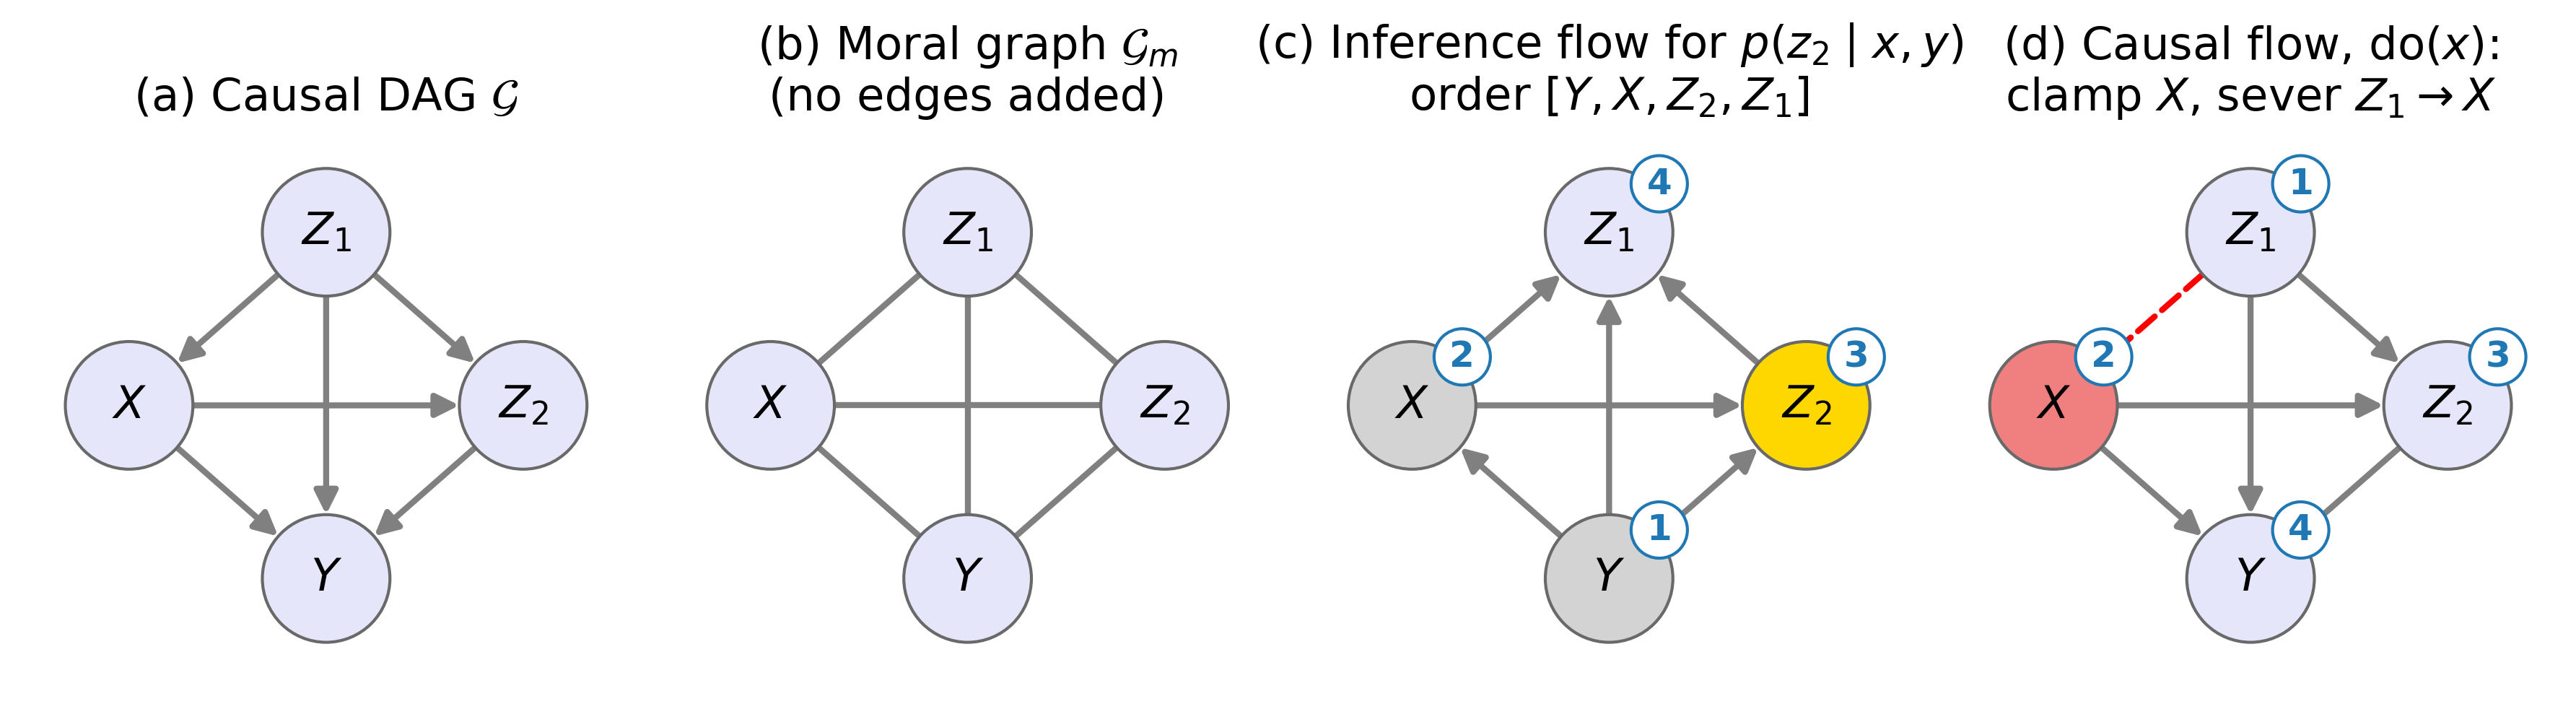
\includegraphics[width=\textwidth]{images/worked_example_compilation.png}
    \caption{\textbf{Worked example of the compiler.} \textbf{(a)}~The causal DAG $\mathcal{G}$. \textbf{(b)}~Its moral graph $\mathcal{G}_m$: every pair of parents sharing a child is already adjacent, so moralization adds no edge here (contrast Figure~\ref{fig:dual-flow}, where it does). \textbf{(c)}~The inference-aligned flow compiled for $p(z_2 \mid x, y)$: conditions $X, Y$ (gray) precede the target $Z_2$ (gold); the marginalized $Z_1$ is ordered last and is never sampled for this query. Circled numbers give the block order. \textbf{(d)}~The causal-aligned flow answering $p(y \mid \mathrm{do}(x))$: the block of $X$ is clamped (red), severing the edge $Z_1 \to X$ (dashed), while $Z_1$ is integrated from its prior.}
    \label{fig:worked-example}
\end{figure*}

\paragraph{Query 1: $p(z_2 \mid x, y)$ (Inference Alignment).}
The conditions are $\{X, Y\}$ and the target is $\{Z_2\}$; the remaining variable $Z_1$ is neither, and must be marginalized.
\emph{Moralization:} the parents of $Y$ ($\{Z_1, X, Z_2\}$) and of $Z_2$ ($\{Z_1, X\}$) are married pairwise; in this dense graph every such pair is already adjacent, so no edge is added and the moral graph $\mathcal{G}_m$ is the complete graph on the four nodes. (Figure~\ref{fig:dual-flow} shows the complementary case of a bare collider, where moralization does add an edge.)
\emph{Re-ordering:} the conditions come first, sorted in reverse topological order, giving $[Y, X]$; the breadth-first traversal of $\mathcal{G}_m$ then appends $Z_2$ and finally $Z_1$, so $\mathcal{O} = [Y, X, Z_2, Z_1]$. Note that the marginalized variable $Z_1$ lands \emph{after} the target: the prefix $\{Y, X, Z_2\}$ is ancestrally closed in the compiled graph, so by Theorem~\ref{thm:marginalization} the flow marginalizes $Z_1$ for free---it is simply never sampled.
\emph{Pruning:} every candidate dependency is tested by d-separation in $\mathcal{G}$. For instance, $Z_2$'s candidate parents are $\{Y, X\}$: $Z_2 \not\perp_d Y \mid X$ and $Z_2 \not\perp_d X \mid Y$ (both direct edges), so both survive; likewise all of $Z_1$'s candidate parents survive. Nothing is pruned here---pruning takes effect on sparser graphs, removing candidate dependencies between d-separated variables as in Figure~\ref{fig:example-pgm-compilation-41}.
The compiled flow therefore has ordering $[Y, X, Z_2, Z_1]$ with full triangular dependencies. To answer the query, the blocks of $(Y, X)$ are clamped to the observed values and the single block of $Z_2$ is integrated---one ODE solve, no MCMC, and no sampling of $Z_1$.

\paragraph{Query 2: $p(y \mid \mathrm{do}(x))$ (Causal Alignment).}
The causal-alignment model keeps $\mathcal{G}$ unchanged: ordering $[Z_1, X, Z_2, Y]$ with parent sets read directly off the DAG. The intervention clamps the block of $X$ to $x$---severing its dependence on $Z_1$---while $Z_1$ is integrated from its \emph{prior}, then $Z_2$ given $(z_1, x)$, then $Y$ given $(z_1, x, z_2)$. The resulting $y$-marginal is exactly the truncated factorization
\begin{equation}
    p(y \mid \mathrm{do}(x)) = \int p(z_1)\, p(z_2 \mid z_1, x)\, p(y \mid z_1, x, z_2)\, dz_1\, dz_2.
\end{equation}
This example also illustrates the distinction drawn in Section~\ref{sec:experiments}: because $X$ has an ancestor ($Z_1$) outside the conditioning set, $\{X\}$ is not ancestrally closed, so $p(y \mid \mathrm{do}(x)) \neq p(y \mid x)$---the observational conditional would re-weight $Z_1$ by $p(z_1 \mid x)$ through the back-door path $X \leftarrow Z_1 \to Y$. Answering \emph{that} query is the business of a separate inference-aligned compilation with conditions $\{X\}$.

\subsection{Tractability}
For a detailed theoretical derivation of the tractability conditions for marginals and conditionals in Block-Triangular Flows, please refer to Theorem 1 in Appendix~\ref{app:proof}.

\subsection{Examples}

Figures~\ref{fig:example-pgm-compilation-41} and~\ref{fig:example-pgm-compilation-41-6} show compiler outputs for randomly generated graphs at $n=4$ and $n=6$: the given causal DAG (left) and the moralized, re-ordered, pruned inference DAG compiled for the leaf-conditioned posterior (right).

\begin{figure}[hbt!]
    \centering
    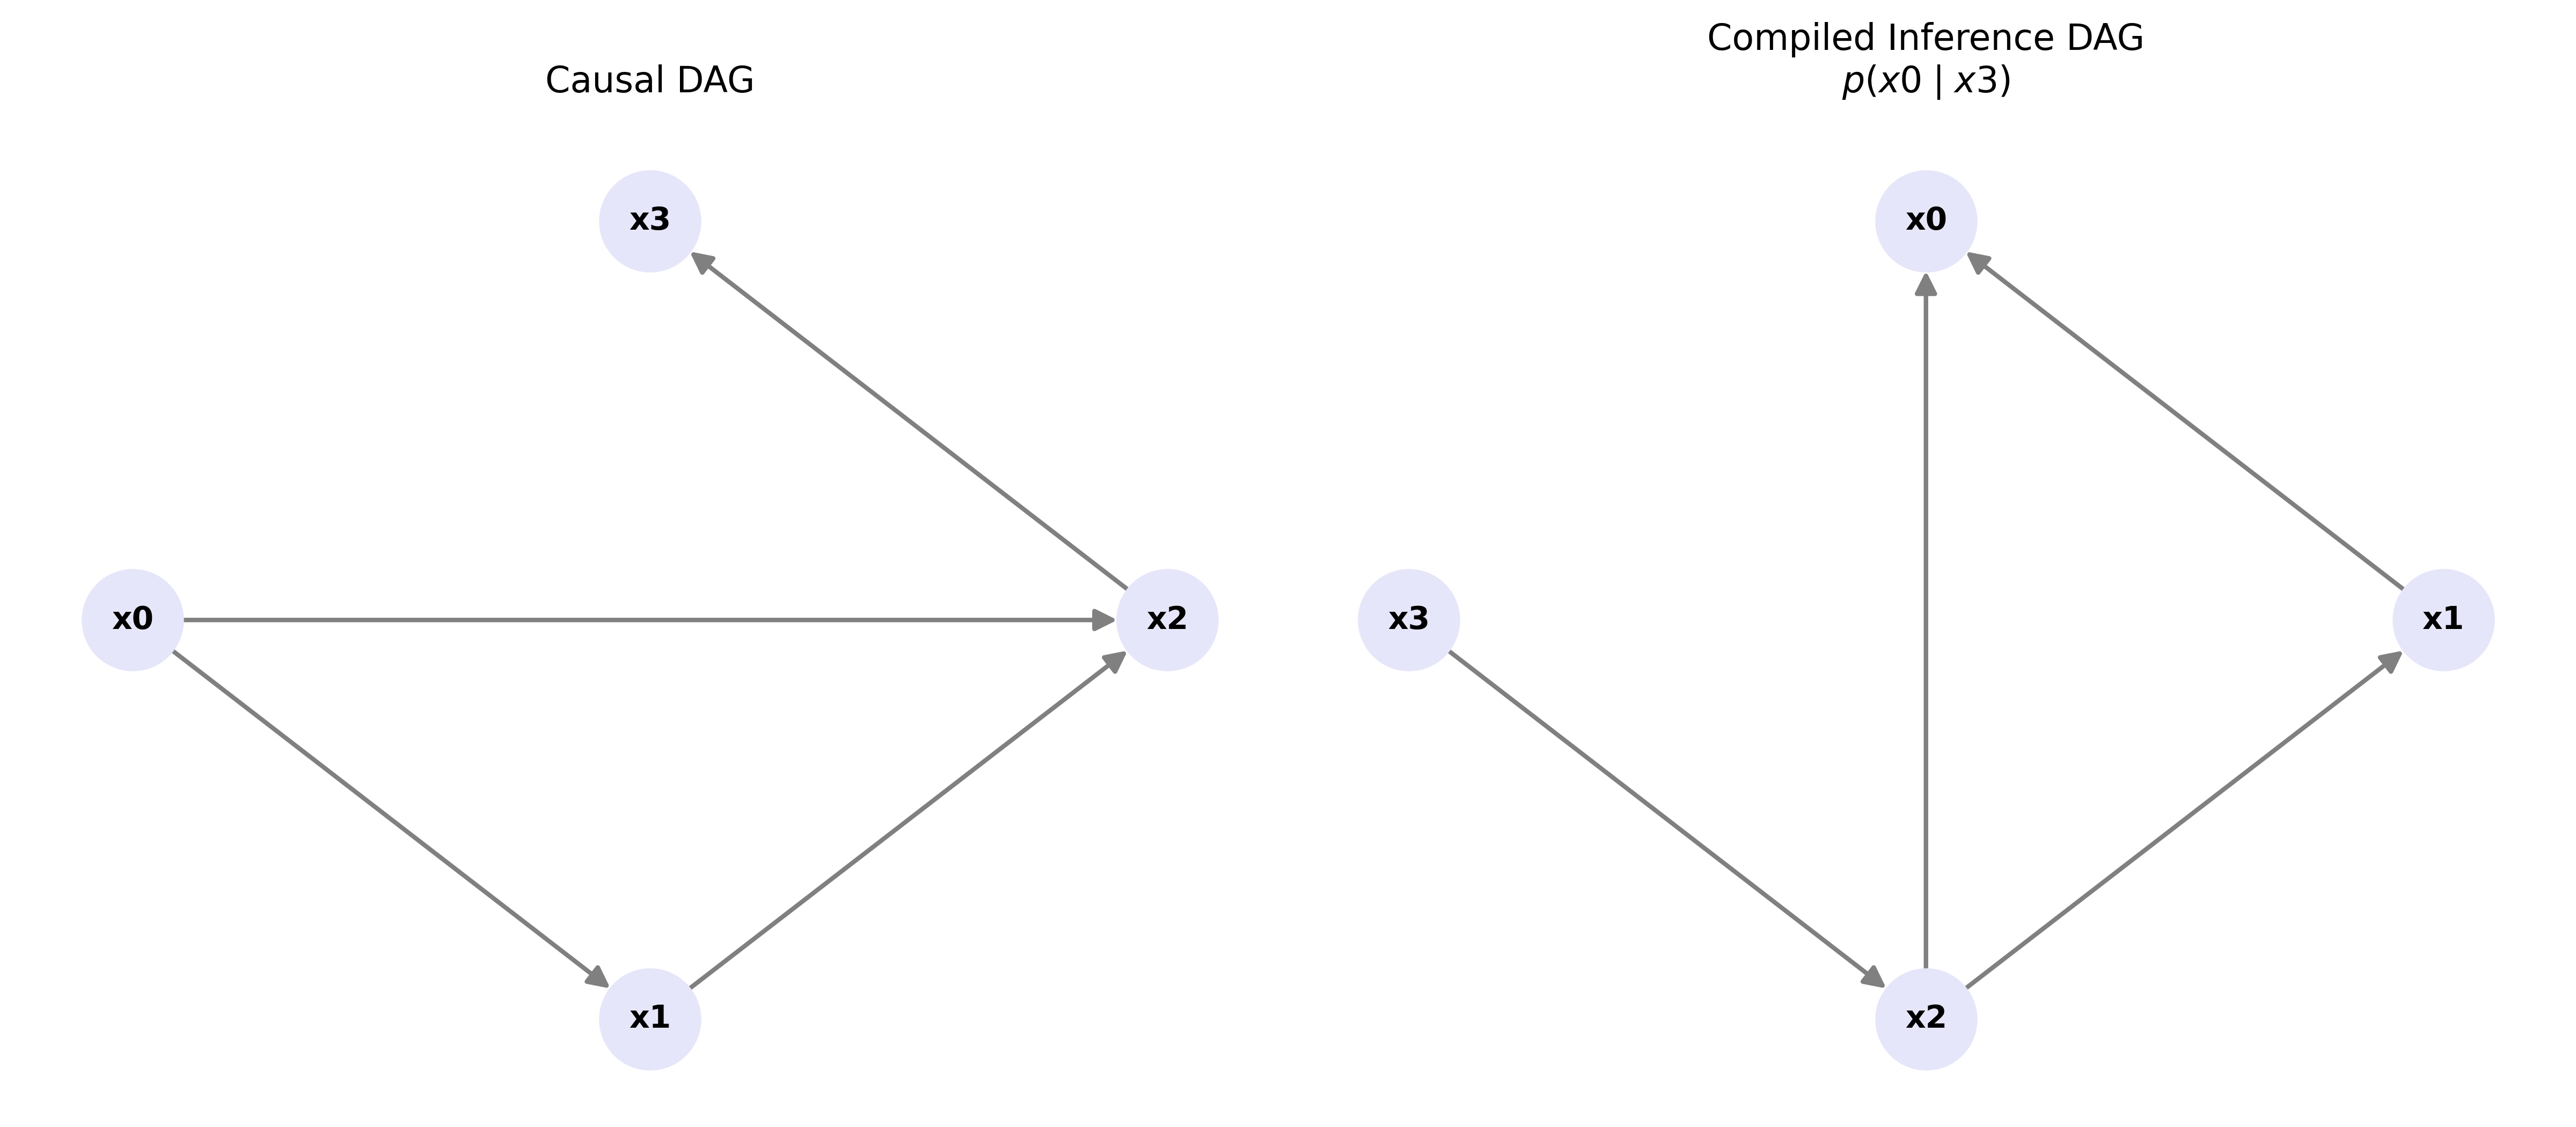
\includegraphics[width=0.68\columnwidth]{images/pgm_compilation_visualization_41_4.png}
    \caption{An example of StructFlow ($n=4$, Seed 41). We start with the given structure / DAG (left), which defines the dependencies of the causally-aligned flow. Alternatively, we compile the structure for inference (right), yielding a different DAG that supports inference queries.}
    \label{fig:example-pgm-compilation-41}
\end{figure}

\begin{figure}[hbt!]
    \centering
    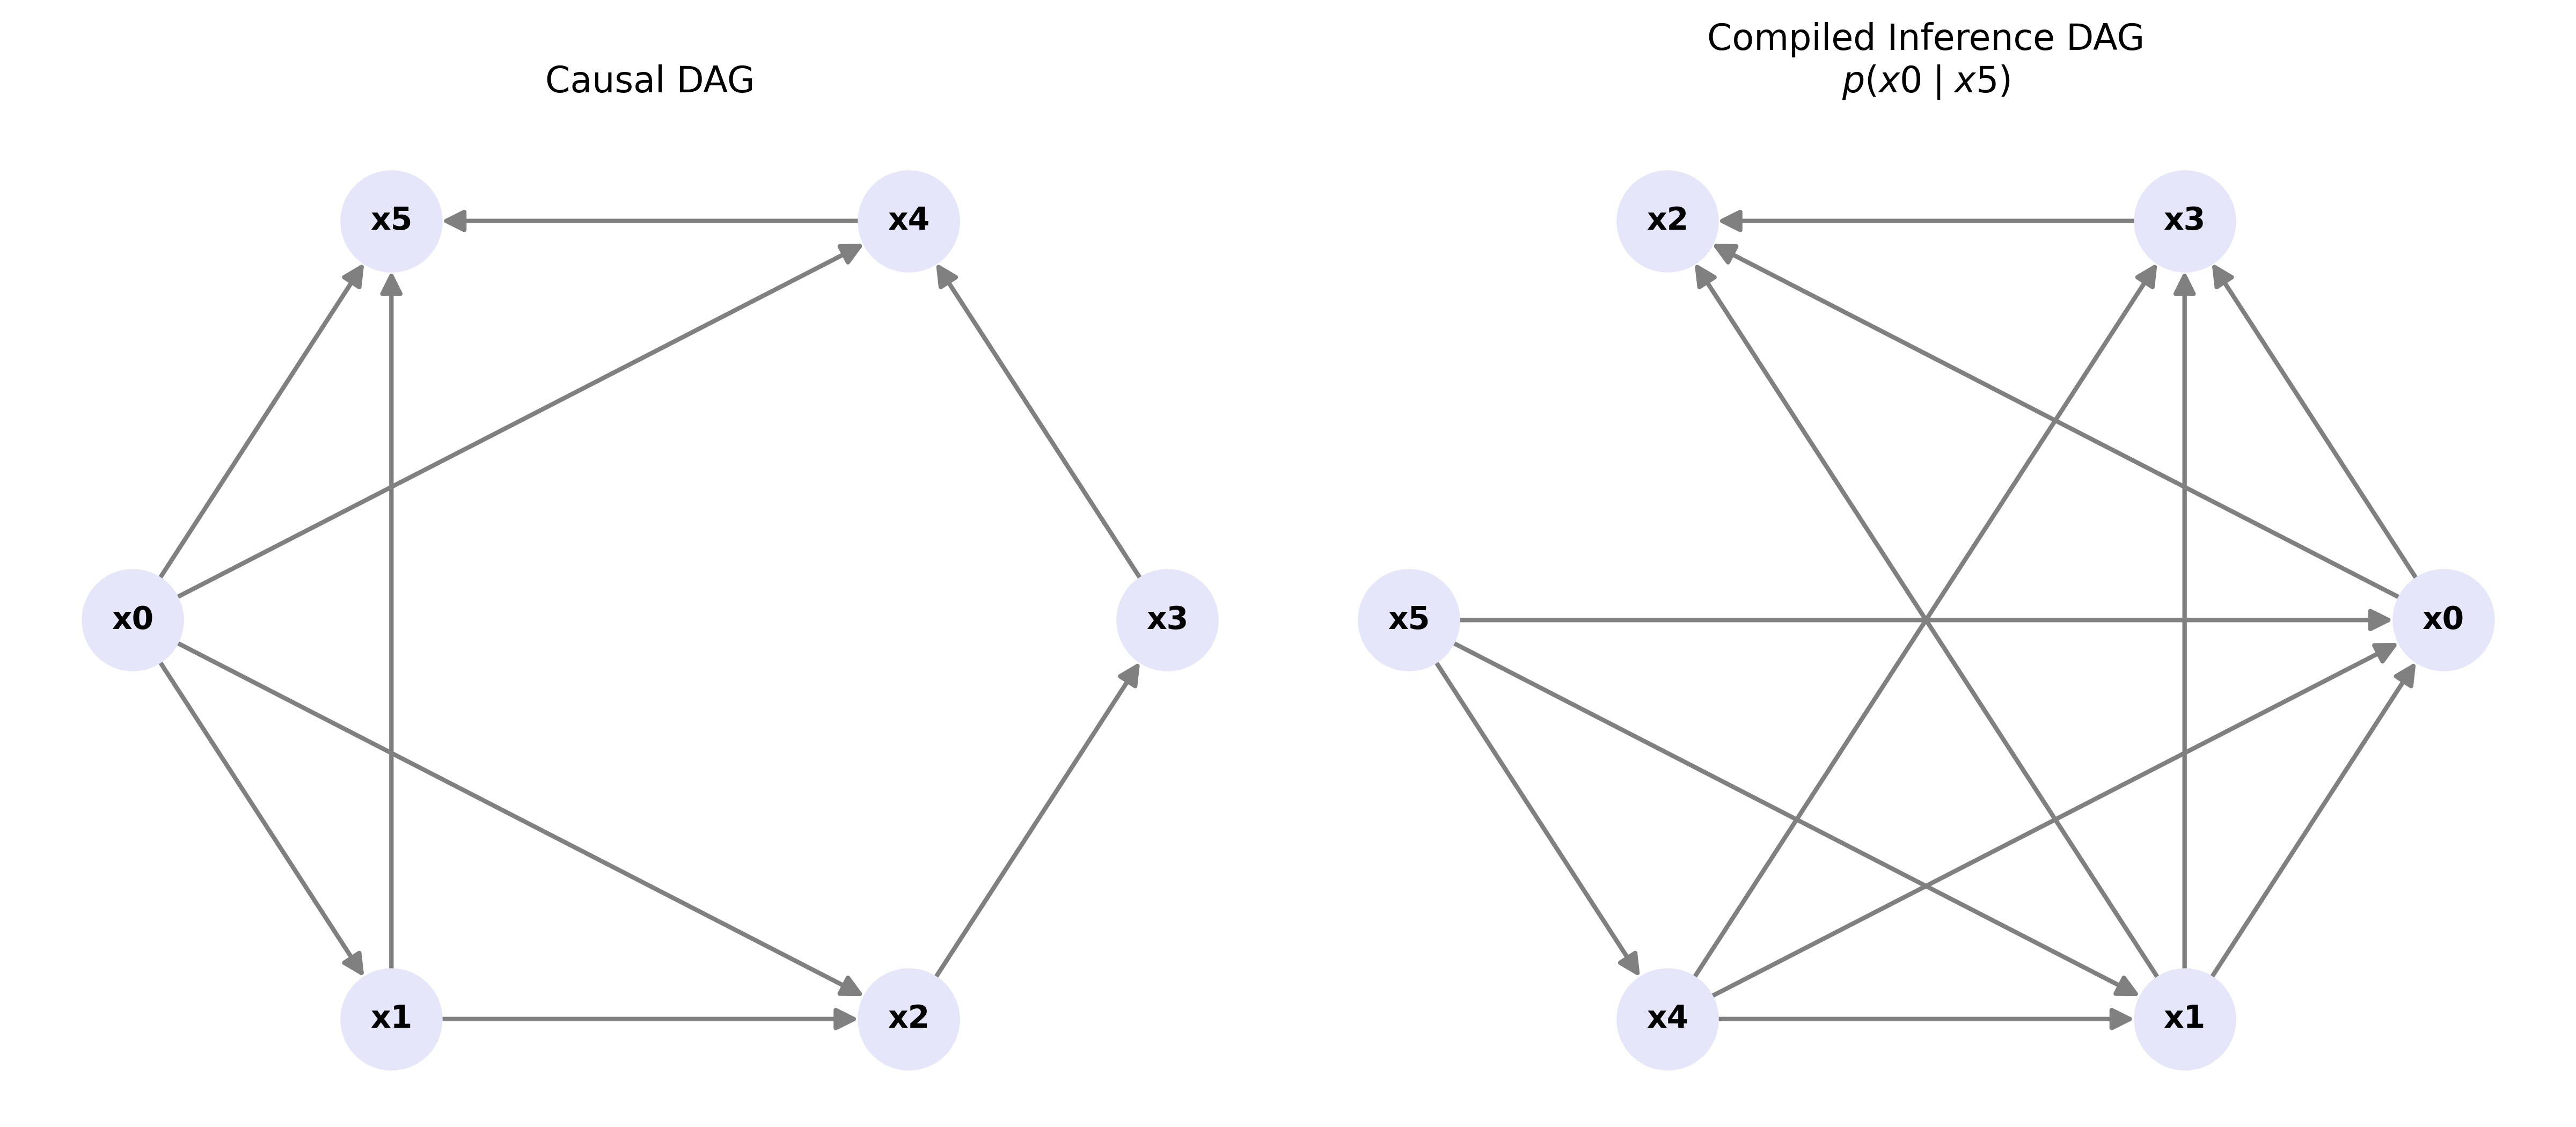
\includegraphics[width=0.68\columnwidth]{images/pgm_compilation_visualization_41_6.png}
    \caption{As Figure~\ref{fig:example-pgm-compilation-41}, for a denser graph ($n=6$, Seed 41).}
    \label{fig:example-pgm-compilation-41-6}
\end{figure}